\documentclass[border=15pt, multi, tikz]{standalone}
\usepackage{import}
\usepackage{etoolbox}
\usepackage{graphicx}
\usepackage{svg}
\usepackage{colortbl}

\usetikzlibrary{positioning,matrix,fit}
\usetikzlibrary{3d} %for including external image
\usetikzlibrary{decorations,shapes}
\usetikzlibrary{decorations.shapes}
\usetikzlibrary{decorations.markings}
\usetikzlibrary{decorations.pathreplacing}
\usetikzlibrary{backgrounds}
\usetikzlibrary{calc}
\usetikzlibrary{arrows.meta,arrows}
\graphicspath{{image/}}

%https://github.com/PetarV-/TikZ


\def\layersep{3cm}
\colorlet{cvTestColor}{red!20}
\colorlet{cvValColor}{yellow!20}
\colorlet{cvTrainColor}{green!20}

\tikzset{%
  >={Latex[width=2mm,length=2mm]},
  % Specifications for style of nodes:
            base/.style = {rectangle, rounded corners, draw=black,
                           minimum width=4cm, minimum height=1cm,
                           text centered, font=\sffamily},
         title/.style = {font=\sffamily},
         process/.style = {base, minimum width=2.5cm, font=\ttfamily, xshift=4cm},
         processFirst/.style = {base, minimum width=2.5cm, font=\ttfamily},
         processModel/.style = {base, minimum width=3cm, minimum height=1.5cm},
         neuron/.style = {circle,fill=black!25,minimum size=5pt,inner sep=0pt},
         inputNeuron/.style = {neuron, fill=green!50},
         outputNeuron/.style = {neuron, fill=red!50},
         hiddenNeuron/.style = {neuron, fill=blue!50},
}
\tikzset{pics/.cd,
  pic mlp/.style={code={
      % Draw the input layer nodes
    \foreach \name / \y in {1,...,4}
    % This is the same as writing \foreach \name / \y in {1/1,2/2,3/3,4/4}
        \node[inputNeuron] (I-\name) at (0,-\y) {};

    % Draw the hidden layer nodes
    \foreach \name / \y in {1,...,5}
        \path[yshift=0.5cm]
            node[hiddenNeuron] (H-\name) at (\layersep,-\y) {};

    % Draw the output layer node
    \node[outputNeuron, right of=H-3,xshift=-10pt] (O) {};

    % Connect every node in the input layer with every node in the
    % hidden layer.
    \foreach \source in {1,...,4}
        \foreach \dest in {1,...,5}
            \path (I-\source) edge (H-\dest);

    % Connect every node in the hidden layer with the output layer
    \foreach \source in {1,...,5}
        \path (H-\source) edge (O);
  }}
}

\begin{document}
\begin{tikzpicture}
    \tikzstyle{every pin edge}=[<-,shorten <=1pt];
    \tikzstyle{annot} = [text width=4em, text centered];
    
  \node (subject) [processFirst] {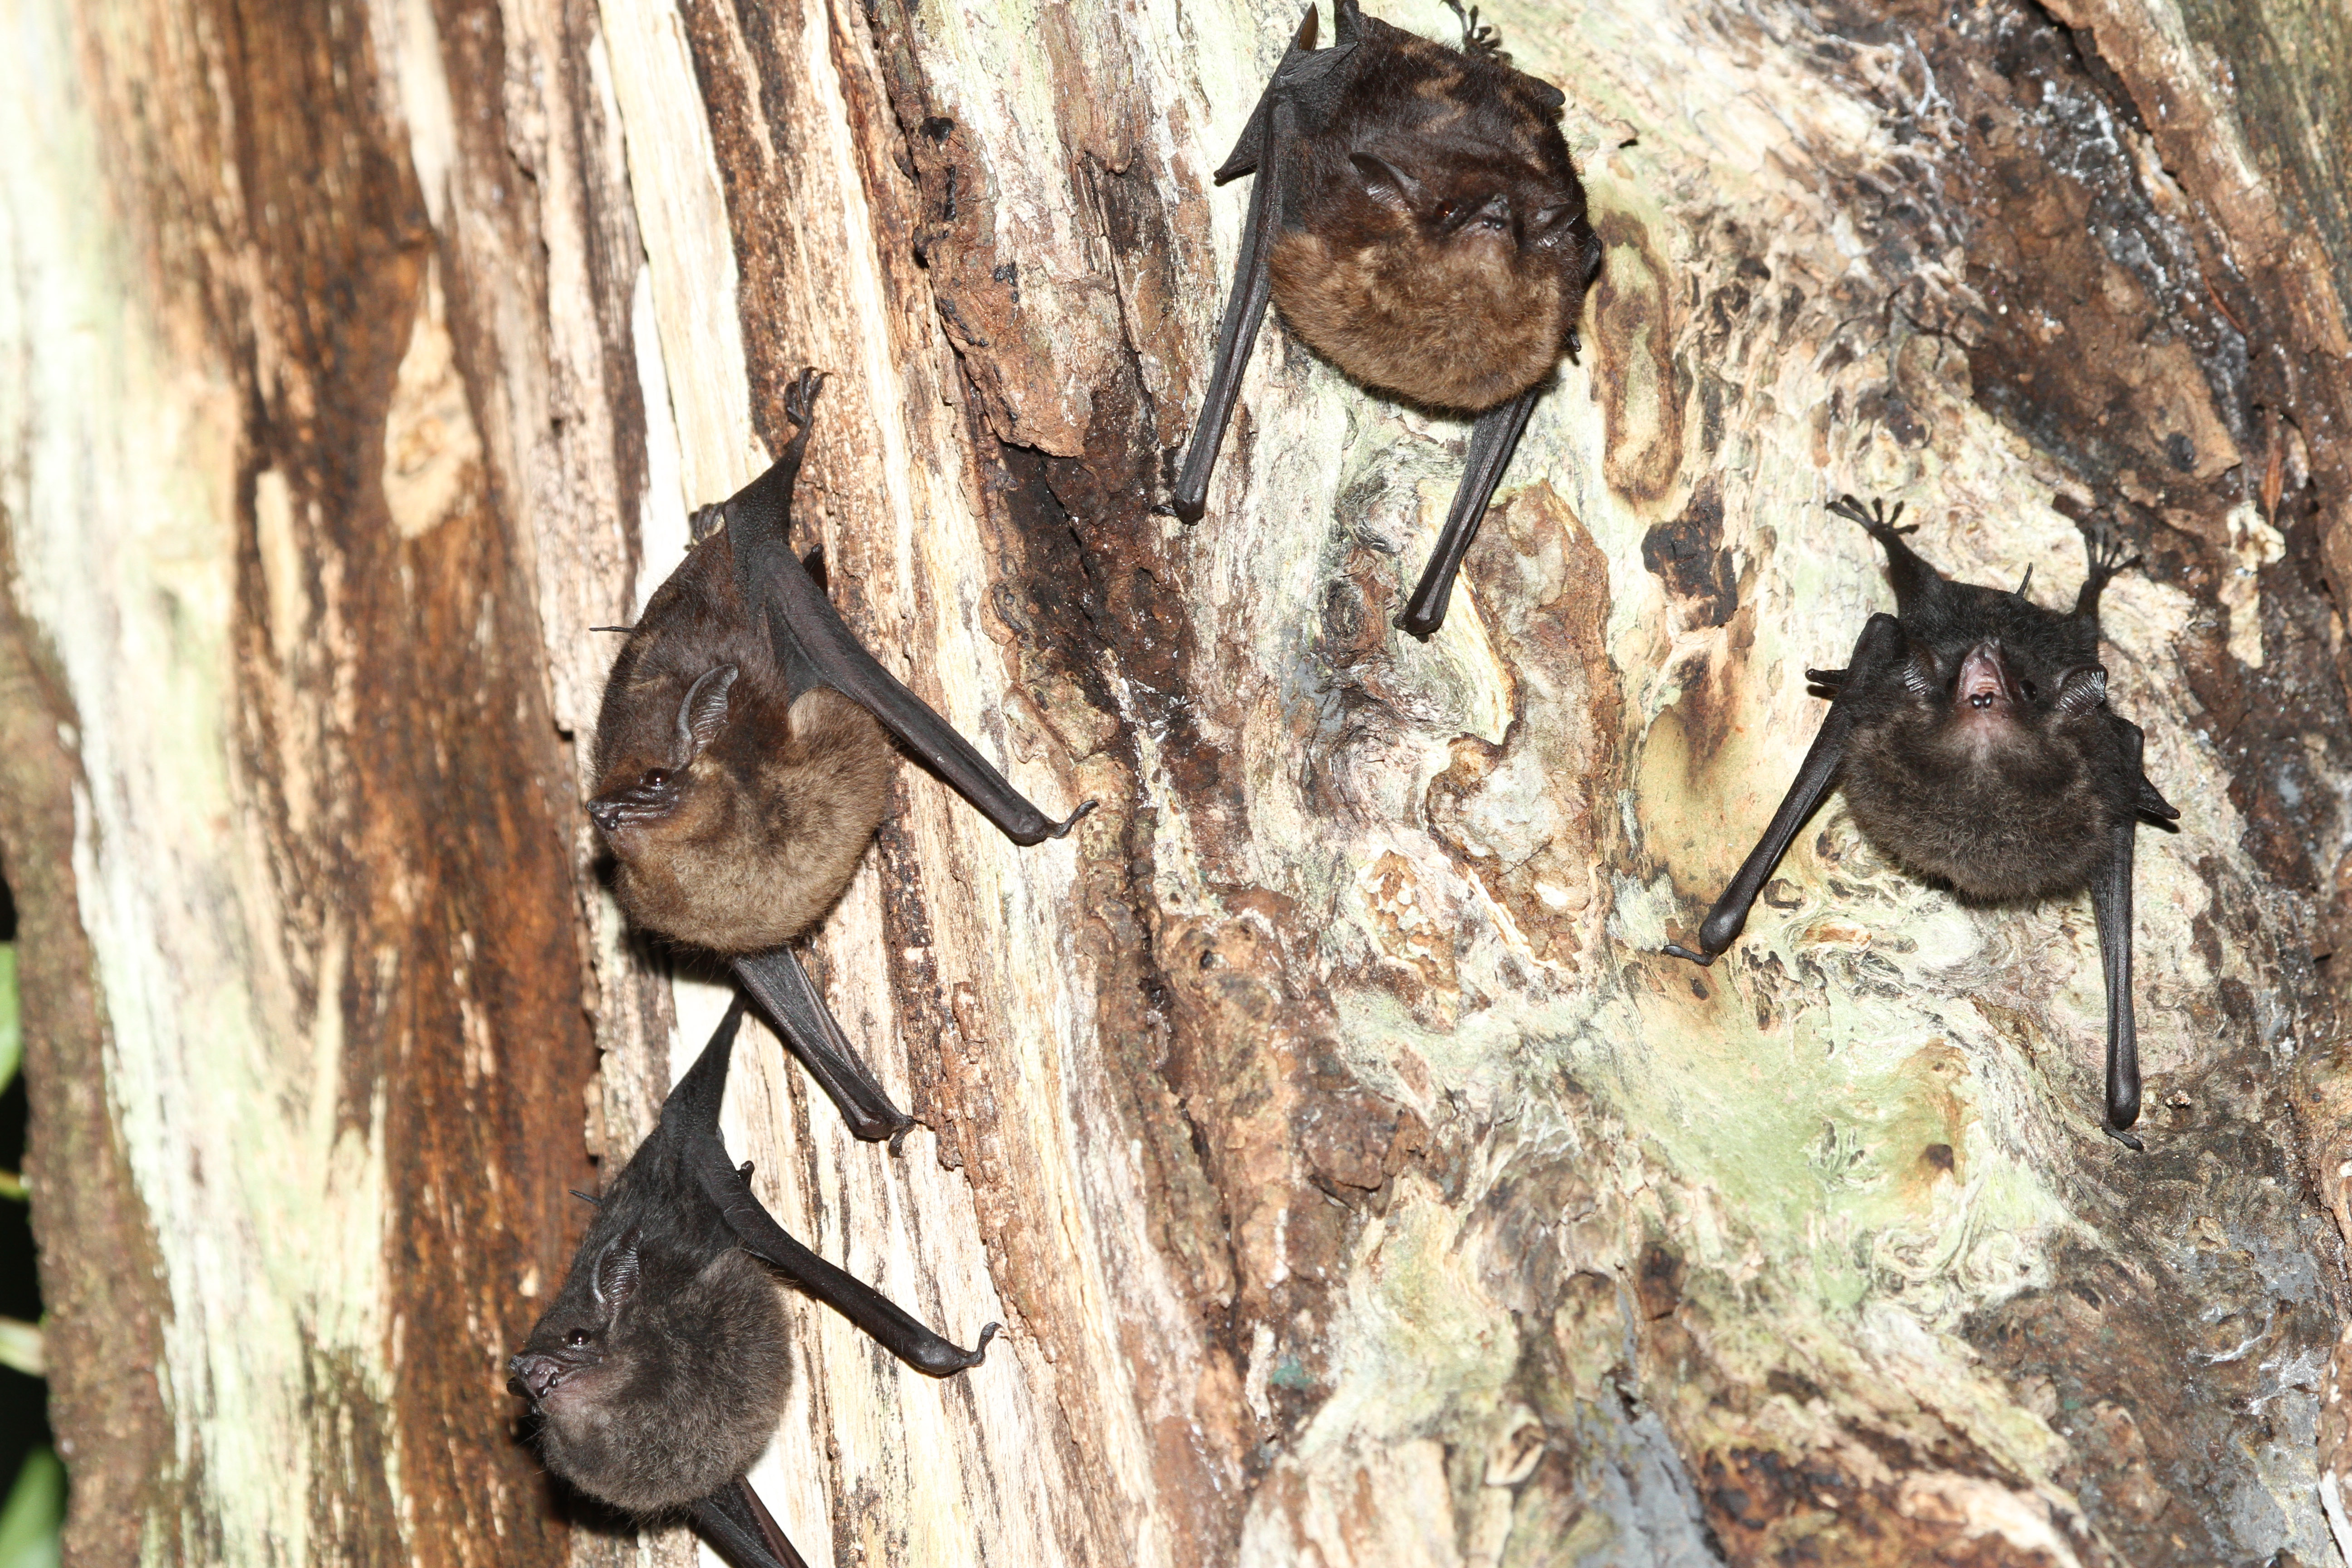
\includegraphics[width=3cm]{Sacco Dayroost.jpg}};
  \node (recording) [process, right of=subject] {\includesvg[inkscapelatex=false,width=2.5cm]{pipline_audio_waveform.svg}};
  \node (preprocessing) [process, right of=recording] {\includesvg[inkscapelatex=false,width=2.5cm]{pipline_audio_spectrogram.svg}};
%   \node (features)  [process, right of=preprocessing,scale=.5,ampersand replacement=\&] {
%     \begin{tabular}{c c c c}
%         0.01 & 0.04 & 0.2 & 0.5 \\
%         0.5 & 0.01 & 0.04 & 0.2 \\
%         0.1 & 0.01 & 0.04 & 0.2 \\
%         0.9 & 0.31 & 0.84 & 0.62 \\
%     \end{tabular}
%   };
  
    \node (features)  [process, right of=preprocessing, scale=.75,ampersand replacement=\&] {
    \begin{tabular}{c c c c}
        \multicolumn{2}{c}{\cellcolor{cvTrainColor}Train} & \cellcolor{cvValColor}Val & \cellcolor{cvTestColor}Test \\
        \cellcolor{cvTestColor}Test & \multicolumn{2}{c}{\cellcolor{cvTrainColor}Train} & \cellcolor{cvValColor}Val \\
        \cellcolor{cvValColor}Val & \cellcolor{cvTestColor}Test & \multicolumn{2}{c}{\cellcolor{cvTrainColor}Train} \\
    \end{tabular}
  };
  
  \node (train) [processModel, below of=preprocessing, yshift=-1.25cm]{};
  \pic[scale=.25,shift={(100pt, -10pt)}] at (train.north west) {pic mlp};
  
  \node (test) [processModel, below of=train, yshift=-1.25cm]{};
  \pic[scale=.25,shift={(100pt, -10pt)}] at (test.north west) {pic mlp};
  
  \node [title, above of=subject, yshift=5mm]{Subject};
  \node [title, above of=recording]{Audio};
  \node [title, above of=preprocessing]{Spectrogram};
  \node [title, above of=features]{Features};
  \node [title, above of=train]{Train Model};
  \node [title, below of=test]{Test Model};
  
  \draw[->] (subject) -- (recording) node[midway,above] {Recording};
  \draw[->] (recording) -- (preprocessing) node[midway,above] {Processing};
  \draw[->] (preprocessing) -- (features) node[midway,above] {Extracting};
%   \draw[->,out=235, in=45] (features.south) to node[midway,above]{input} (model.north);
  \draw[->,out=270,in=0] (features.south) to node[midway,left,xshift=10pt,yshift=10pt]{input[\colorbox{cvTrainColor}{train},\colorbox{cvValColor}{val}]} (train.east);
  \draw[->,out=270,in=0] (features.south) to node[midway,left]{input[\colorbox{cvTestColor}{test}]} (test.east);
  \draw[->] (train.south) -- (test.north) node[midway,left] {Maturated model};
\end{tikzpicture}
\end{document}\grid